\documentclass[aspectratio=169,10pt]{ctexbeamer}

\usetheme{Madrid}
\usecolortheme{default}
\setbeamertemplate{navigation symbols}{}
\setbeamertemplate{footline}[frame number]

\usepackage{amsmath}
\usepackage{booktabs}
\usepackage{array}
\usepackage{graphicx}
\usepackage{tikz}
\usepackage{xcolor}
\usepackage{listings}
\usetikzlibrary{arrows.meta, positioning}

\definecolor{ucasblue}{RGB}{30,70,120}
\definecolor{ucasgreen}{RGB}{36,120,92}
\definecolor{lightgray}{RGB}{245,247,250}
\definecolor{codeblue}{RGB}{28,68,135}
\definecolor{codegreen}{RGB}{40,120,80}

\setbeamercolor{structure}{fg=ucasblue}
\setbeamercolor{title}{fg=white,bg=ucasblue}
\setbeamercolor{frametitle}{fg=white,bg=ucasblue}
\setbeamercolor{block title}{fg=white,bg=ucasblue}
\setbeamercolor{block body}{bg=lightgray}
\setbeamerfont{frametitle}{series=\bfseries}
\setbeamerfont{title}{series=\bfseries,size=\Large}

\newcolumntype{M}[1]{>{\centering\arraybackslash}m{#1}}
\graphicspath{{../Figure/}}

\lstset{
	language=Python,
	basicstyle=\ttfamily\scriptsize,
	numbers=left,
	numberstyle=\tiny\color{ucasgreen},
	showstringspaces=false,
	breaklines=true,
	frame=single,
	rulecolor=\color{ucasblue!45},
	framerule=0.4pt,
	backgroundcolor=\color{lightgray},
	columns=fullflexible,
	keywordstyle=\bfseries\color{codeblue},
	commentstyle=\itshape\color{codegreen},
	stringstyle=\color{red!65!black},
	tabsize=4
}

\title{实验二：基于ViT的CIFAR10图像分类}
\subtitle{Vision Transformer on CIFAR10}
\author{尧祥临 \quad 202518023406038}
\institute{中国科学院大学 \quad 前沿交叉科学学院\\2026年春季学期\quad 深度学习}
\date{}

\begin{document}

\begin{frame}
	\titlepage
\end{frame}

\begin{frame}{实验任务}
	\begin{block}{目标}
		从零实现一个基于 ViT 的 CIFAR10 图像分类模型，完成数据读取、网络构建、模型训练和测试评估。
	\end{block}

	\begin{columns}[T,onlytextwidth]
		\begin{column}{0.48\textwidth}
			\textbf{实验要求}
			\begin{itemize}
				\item 使用深度学习框架完成完整训练流程
				\item 构建 ViT 模型和 Attention 结构
				\item 测试集准确率达到 80\% 以上
			\end{itemize}
		\end{column}
		\begin{column}{0.48\textwidth}
			\textbf{本次结果}
			\begin{itemize}
				\item 训练日志共 176 个 epoch
				\item 最高测试准确率：\textbf{85.79\%}
				\item 验证最优模型测试准确率：\textbf{85.61\%}
			\end{itemize}
		\end{column}
	\end{columns}
\end{frame}

\begin{frame}{数据集与划分}
	\begin{columns}[T,onlytextwidth]
		\begin{column}{0.55\textwidth}
			\begin{itemize}
				\item 数据集：CIFAR10
				\item 图像尺寸：$3\times 32\times 32$
				\item 类别数：10类
				\item 训练增强：RandomCrop、RandomHorizontalFlip、RandomErasing
				\item 归一化：CIFAR10 mean/std
			\end{itemize}
		\end{column}
		\begin{column}{0.4\textwidth}
			\begin{table}
				\centering
				\begin{tabular}{l r}
					\toprule
					划分 & 样本数 \\
					\midrule
					训练集 & 45000 \\
					验证集 & 5000 \\
					测试集 & 10000 \\
					\bottomrule
				\end{tabular}
			\end{table}
		\end{column}
	\end{columns}

	\vspace{0.25cm}
	\begin{block}{划分方式}
		使用固定随机种子 114514 从官方训练集中划分训练集和验证集，官方测试集保持不变。
	\end{block}
\end{frame}

\begin{frame}{整体流程}
	\centering
	\begin{tikzpicture}[
		node distance=0.45cm,
		flowstep/.style={draw=ucasblue, fill=lightgray, rounded corners=2pt,
			minimum width=2.35cm, minimum height=0.78cm, align=center},
		arrow/.style={-{Latex[length=2mm]}, thick, draw=ucasblue}
	]
		\node[flowstep] (data) {CIFAR10\\增强与归一化};
		\node[flowstep, right=of data] (patch) {Patch\\Embedding};
		\node[flowstep, right=of patch] (encoder) {Transformer\\Encoder};
		\node[flowstep, right=of encoder] (train) {AdamW + EMA\\Mixup 训练};
		\node[flowstep, right=of train] (eval) {验证集选择\\测试评估};
		\draw[arrow] (data) -- (patch);
		\draw[arrow] (patch) -- (encoder);
		\draw[arrow] (encoder) -- (train);
		\draw[arrow] (train) -- (eval);
	\end{tikzpicture}

	\vspace{0.8cm}
	\begin{columns}[T,onlytextwidth]
		\begin{column}{0.48\textwidth}
			\textbf{训练阶段}
			\begin{itemize}
				\item Mixup + label smoothing
				\item 梯度裁剪与DropPath正则化
			\end{itemize}
		\end{column}
		\begin{column}{0.48\textwidth}
			\textbf{评估阶段}
			\begin{itemize}
				\item 使用EMA模型计算验证/测试指标
				\item 按验证集准确率保存最优模型
			\end{itemize}
		\end{column}
	\end{columns}
\end{frame}

\begin{frame}{ViT 模型结构}
	\centering
	\resizebox{\linewidth}{!}{%
	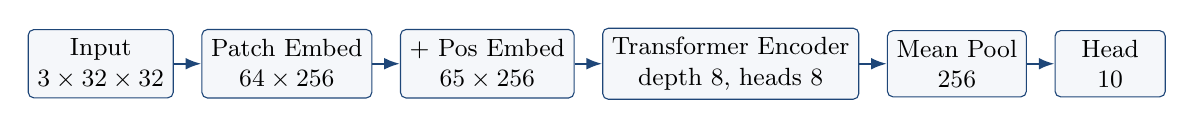
\begin{tikzpicture}[
		layer/.style={draw=ucasblue, fill=lightgray, rounded corners=2pt,
			minimum height=0.8cm, align=center, font=\small},
		arrow/.style={-{Latex[length=2mm]}, thick, draw=ucasblue},
		node distance=0.35cm
	]
		\node[layer, minimum width=1.6cm] (input) {Input\\$3\times32\times32$};
		\node[layer, minimum width=1.9cm, right=of input] (patch) {Patch Embed\\$64\times256$};
		\node[layer, minimum width=1.9cm, right=of patch] (pos) {+ Pos Embed\\$65\times256$};
		\node[layer, minimum width=2.4cm, right=of pos] (trans) {Transformer Encoder\\depth 8, heads 8};
		\node[layer, minimum width=1.6cm, right=of trans] (pool) {Mean Pool\\256};
		\node[layer, minimum width=1.4cm, right=of pool] (out) {Head\\10};
		\foreach \a/\b in {input/patch,patch/pos,pos/trans,trans/pool,pool/out}
			\draw[arrow] (\a) -- (\b);
	\end{tikzpicture}
	}

	\vspace{0.55cm}
	\begin{columns}[T,onlytextwidth]
		\begin{column}{0.48\textwidth}
			\begin{block}{Patch划分}
				$32\times32$ 图像使用 $4\times4$ patch，因此得到 $8\times8=64$ 个patch token。
			\end{block}
		\end{column}
		\begin{column}{0.48\textwidth}
			\begin{block}{分类方式}
				Transformer输出后，对patch token求均值，再送入线性分类头输出10类logits。
			\end{block}
		\end{column}
	\end{columns}
\end{frame}

\begin{frame}[fragile]{Patch Embedding 核心代码}
\begin{lstlisting}
class Embedding(nn.Module):
    def __init__(self, image_size=32, patch_size=4,
                 in_channels=3, embed_dim=256):
        super().__init__()
        self.num_patches = (image_size // patch_size) ** 2
        self.embedding = nn.Sequential(
            nn.Conv2d(in_channels, embed_dim,
                      kernel_size=patch_size,
                      stride=patch_size,
                      bias=False),
            nn.Flatten(2)
        )

    def forward(self, x):
        output = self.embedding(x)
        output = output.transpose(1, 2)
        return output
\end{lstlisting}
\end{frame}

\begin{frame}{Transformer Encoder}
	\begin{columns}[T,onlytextwidth]
		\begin{column}{0.48\textwidth}
			\begin{block}{Self-Attention}
				\[
					\mathrm{Attention}(Q,K,V)
					=\mathrm{softmax}\left(\frac{QK^\top}{\sqrt{d_k}}\right)V
				\]
			\end{block}
			\begin{itemize}
				\item embedding dim = 256
				\item heads = 8
				\item 每个head维度为32
			\end{itemize}
		\end{column}
		\begin{column}{0.48\textwidth}
			\begin{block}{Encoder Layer}
				\begin{itemize}
					\item LayerNorm + MultiheadAttention
					\item 残差连接 + DropPath
					\item LayerNorm + MLP
					\item MLP hidden dim = 1024
				\end{itemize}
			\end{block}
		\end{column}
	\end{columns}
\end{frame}

\begin{frame}{模型规模与训练配置}
	\begin{columns}[T,onlytextwidth]
		\begin{column}{0.48\textwidth}
			\begin{table}
				\centering
				\small
				\begin{tabular}{l r}
					\toprule
					模块 & 参数量 \\
					\midrule
					Patch Embedding & 12288 \\
					Transformer Encoder & 6318080 \\
					Classification Head & 2570 \\
					\midrule
					总计 & 6350346 \\
					\bottomrule
				\end{tabular}
			\end{table}
		\end{column}
		\begin{column}{0.48\textwidth}
			\begin{table}
				\centering
				\small
				\begin{tabular}{l l}
					\toprule
					项目 & 设置 \\
					\midrule
					Batch size & 128 \\
					Learning rate & $4\times10^{-4}$ \\
					Weight decay & $2\times10^{-2}$ \\
					Depth / Heads & 8 / 8 \\
					Drop path & 0.1 \\
					Max epochs & 200 \\
					Stop epoch & 176 \\
					\bottomrule
				\end{tabular}
			\end{table}
		\end{column}
	\end{columns}
\end{frame}

\begin{frame}{训练技巧}
	\begin{columns}[T,onlytextwidth]
		\begin{column}{0.48\textwidth}
			\begin{block}{数据与损失}
				\begin{itemize}
					\item RandomCrop + RandomHorizontalFlip
					\item RandomErasing
					\item Mixup, $\alpha=0.2$
					\item Label smoothing = 0.05
				\end{itemize}
			\end{block}
		\end{column}
		\begin{column}{0.48\textwidth}
			\begin{block}{优化与稳定性}
				\begin{itemize}
					\item AdamW分组权重衰减
					\item EMA decay = 0.9998
					\item Warmup + CosineAnnealingLR
					\item Gradient clipping = 1.0
				\end{itemize}
			\end{block}
		\end{column}
	\end{columns}
\end{frame}

\begin{frame}{训练结果：关键节点}
	\begin{table}
		\centering
		\small
		\begin{tabular}{M{1.5cm} M{2cm} M{2cm} M{5.2cm}}
			\toprule
			Epoch & Val Acc & Test Acc & 说明 \\
			\midrule
			50  & 79.58\% & 80.59\% & 已达到实验要求 \\
			100 & 84.58\% & 85.12\% & 进入稳定提升阶段 \\
			131 & 85.46\% & \textbf{85.79\%} & 测试集准确率最高 \\
			136 & \textbf{85.68\%} & 85.61\% & 验证集准确率最高 \\
			176 & 85.32\% & 85.57\% & early stopping停止训练 \\
			\bottomrule
		\end{tabular}
	\end{table}

	\begin{block}{结论}
		验证集最优点与测试集最优点很接近，说明验证集选择没有明显偏离测试趋势。
	\end{block}
\end{frame}

\begin{frame}{训练曲线}
	\centering
	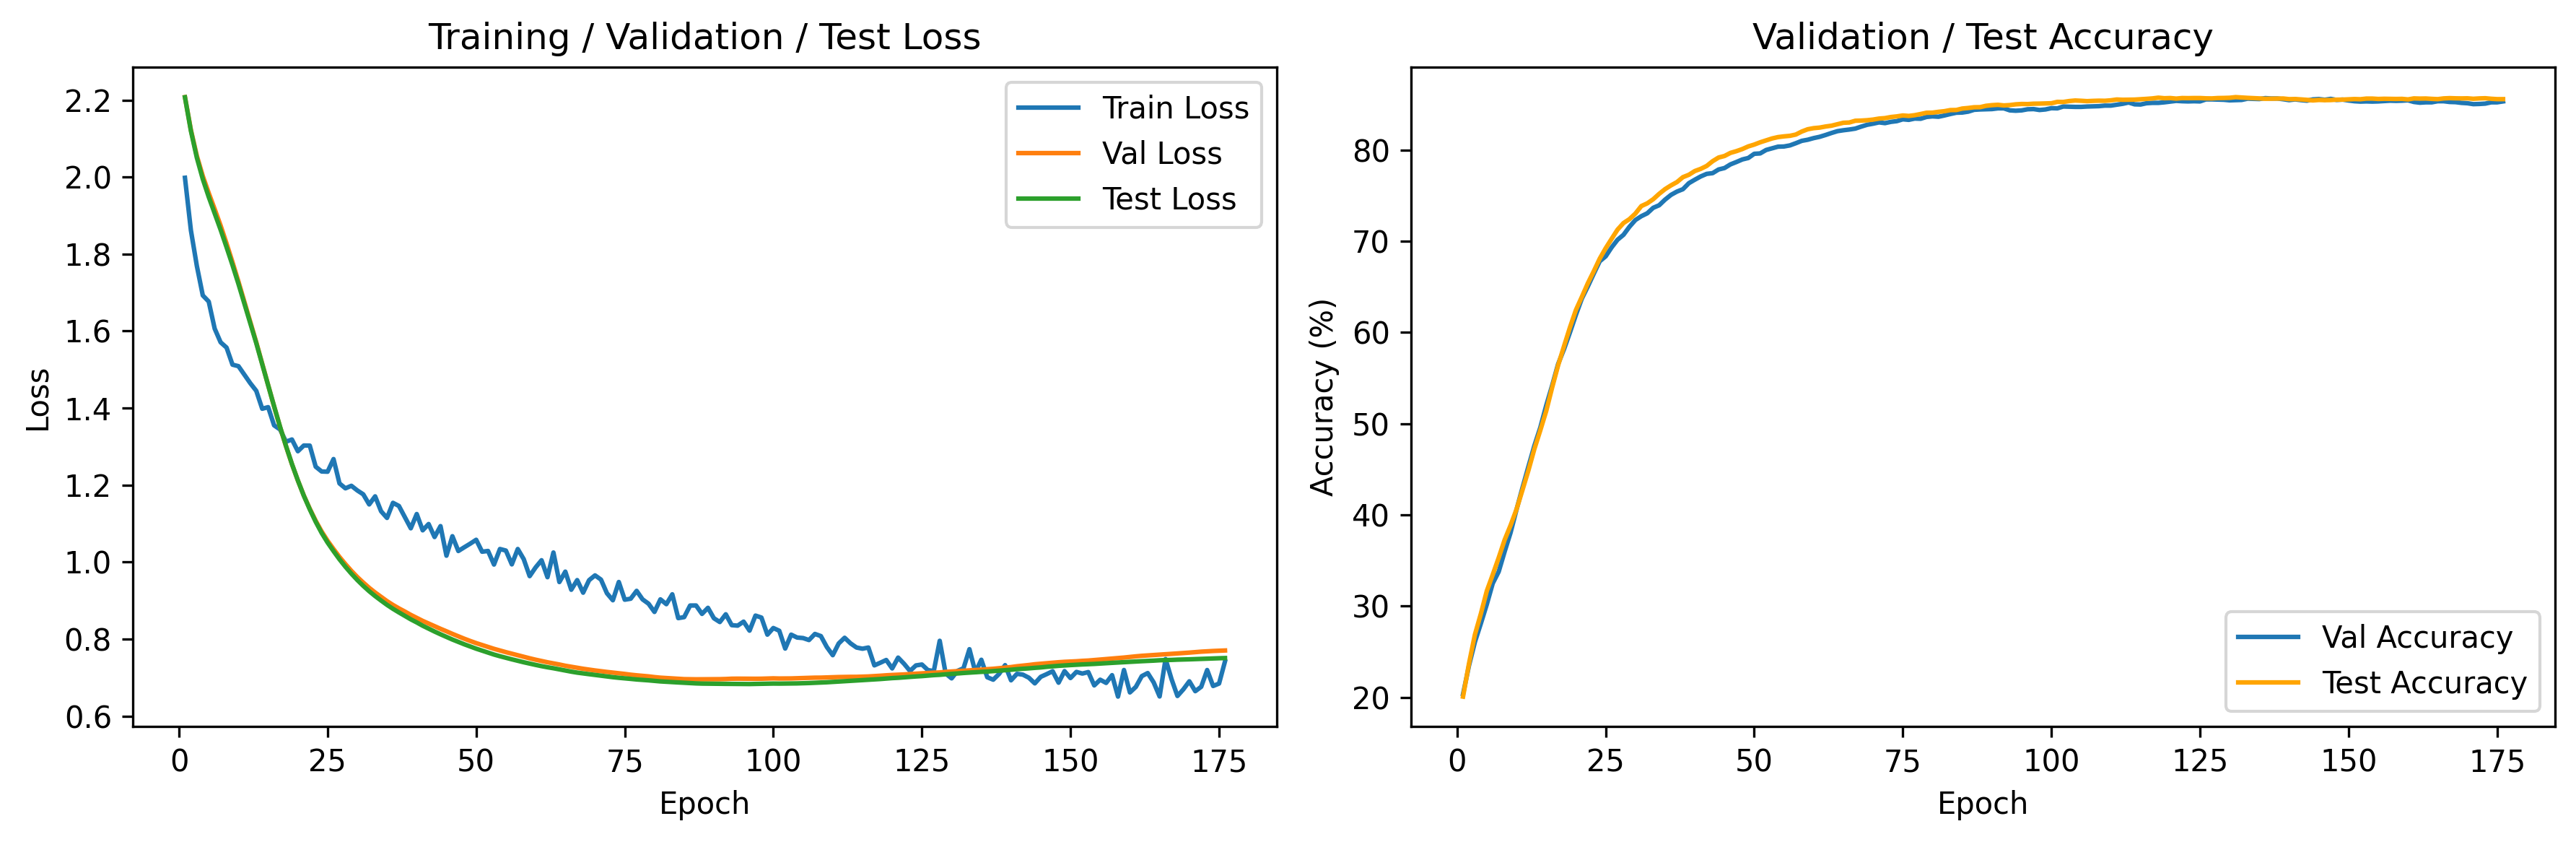
\includegraphics[width=0.94\linewidth]{loss_acc_curves.png}

	\vspace{0.2cm}
	\begin{itemize}
		\item 前50个epoch完成主要拟合，测试准确率达到80.59\%
		\item 50至130个epoch继续缓慢提升，最终稳定在85\%附近
		\item 训练loss后期波动主要来自Mixup和随机增强，不代表验证性能退化
	\end{itemize}
\end{frame}

\begin{frame}{学习率与泛化差距}
	\begin{columns}[T,onlytextwidth]
		\begin{column}{0.50\textwidth}
			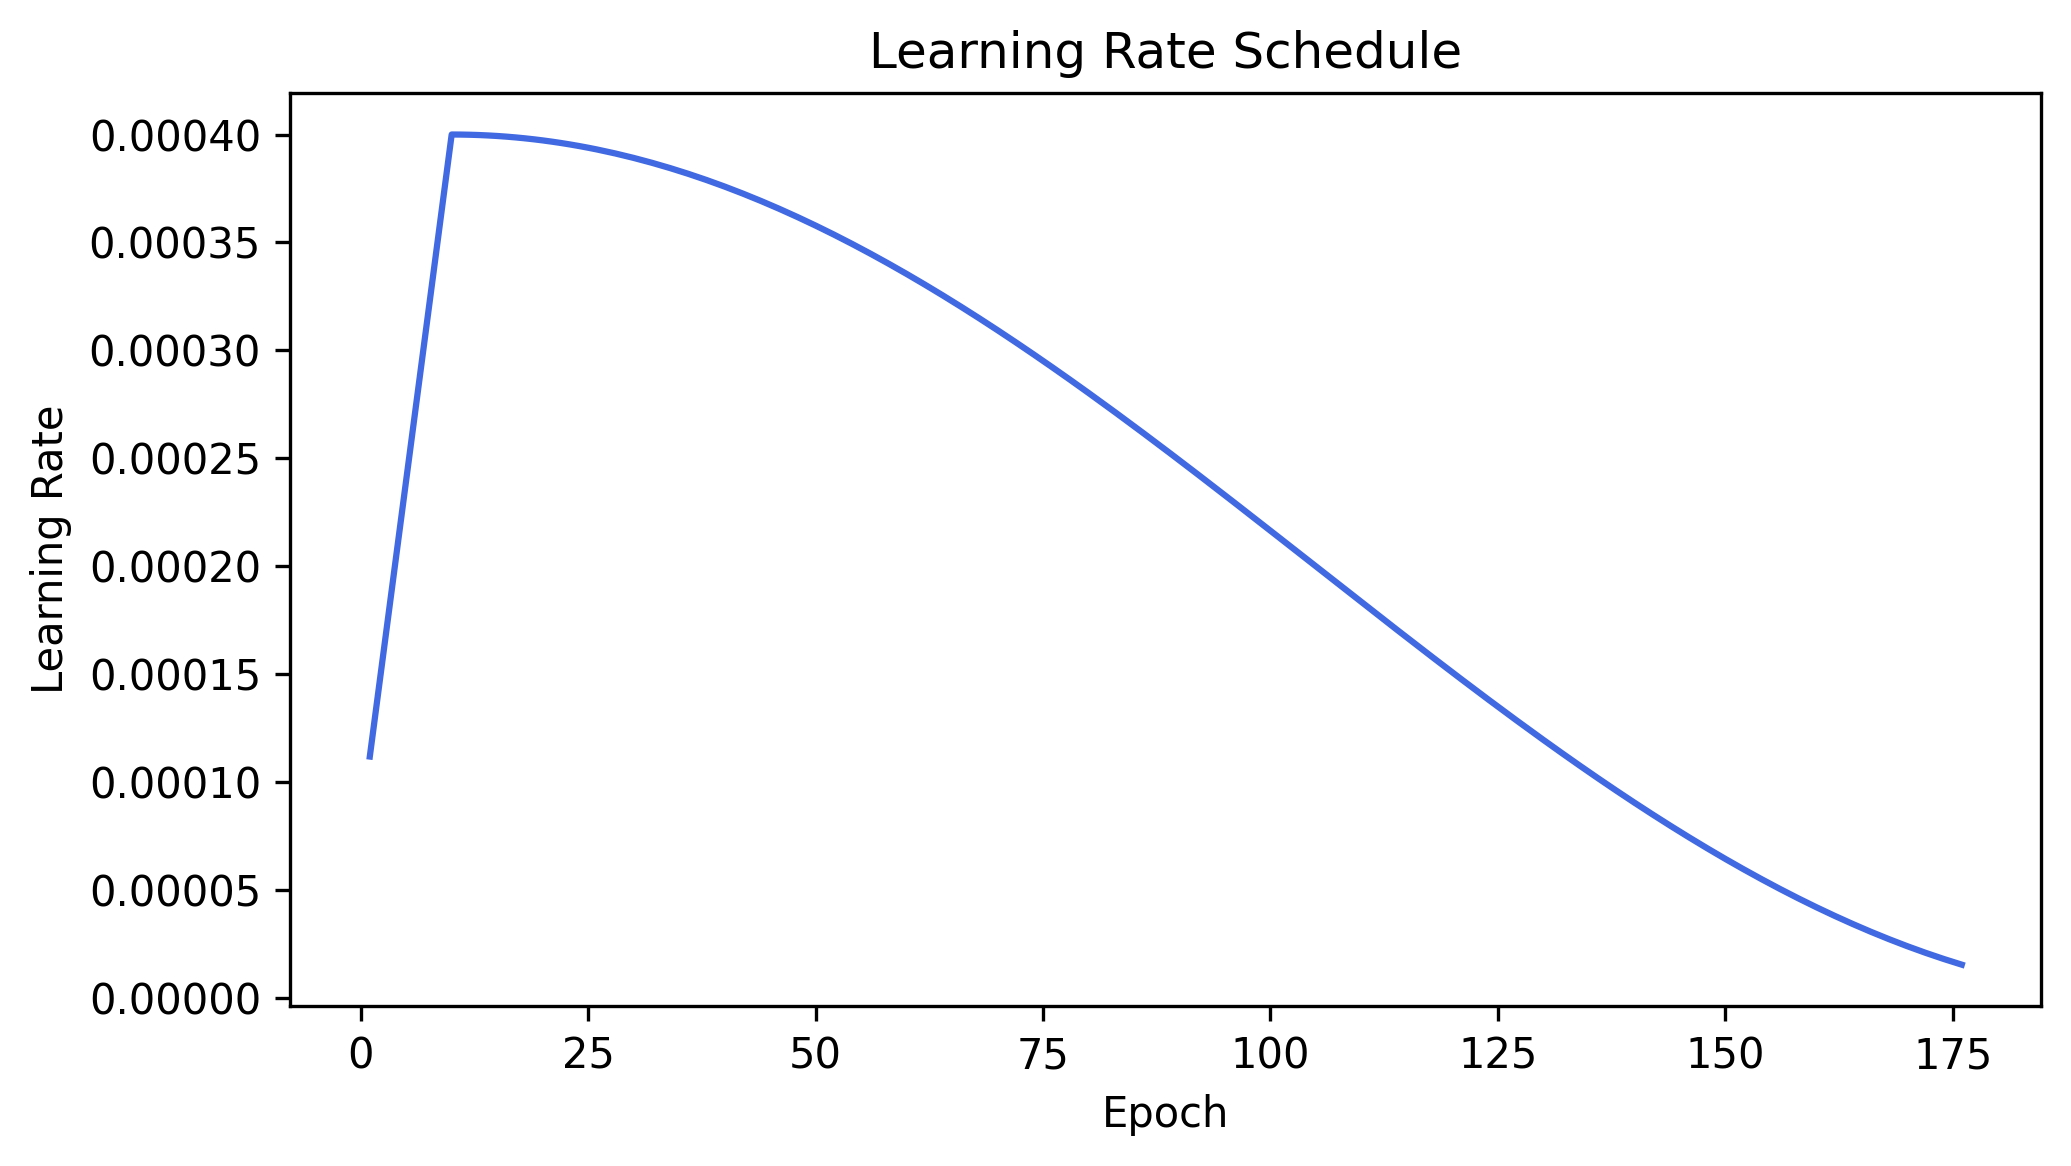
\includegraphics[width=\linewidth]{lr_curve.png}
		\end{column}
		\begin{column}{0.46\textwidth}
			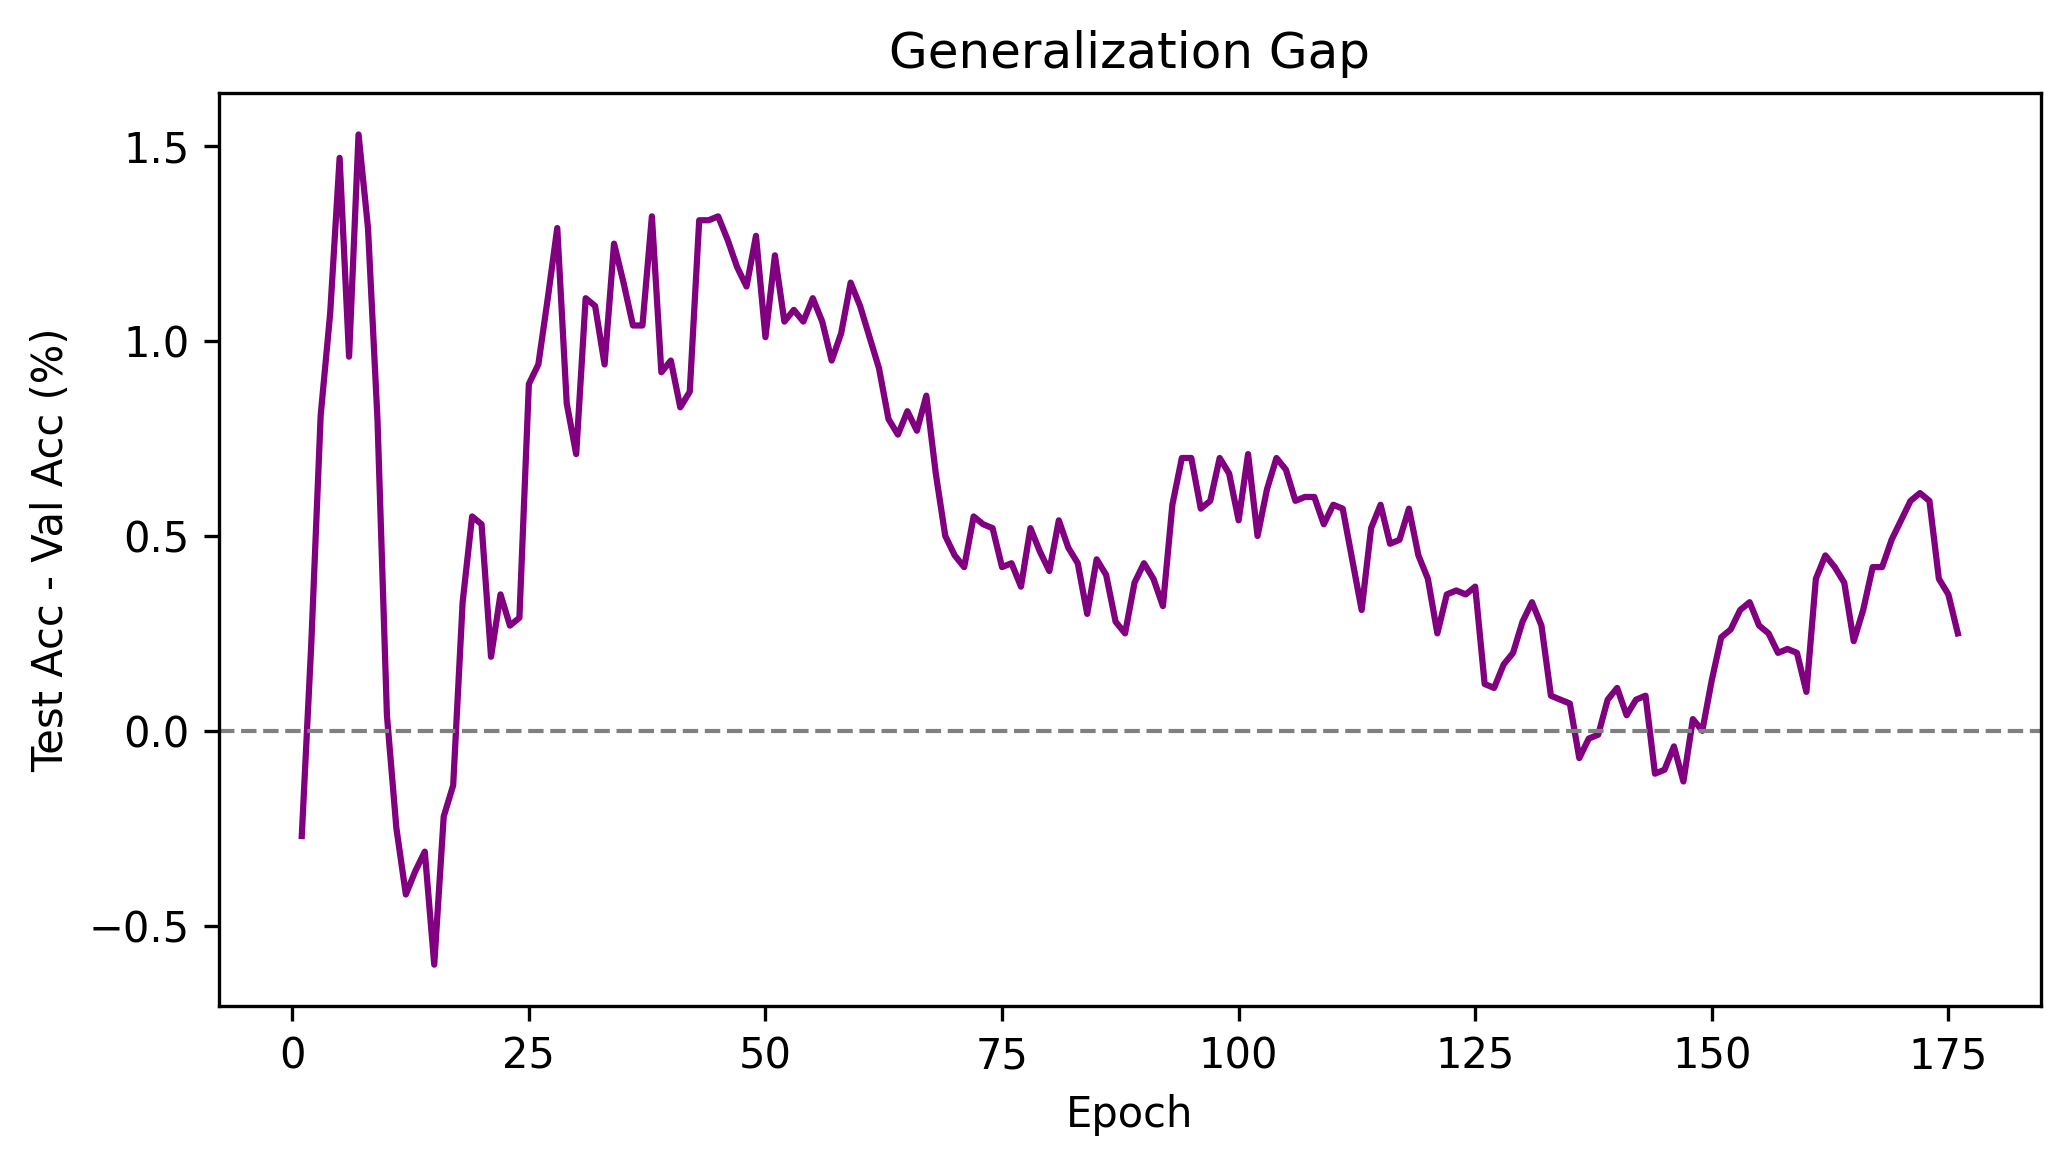
\includegraphics[width=\linewidth]{generalization_gap.png}
			\vspace{0.2cm}
			\begin{itemize}
				\item warmup后余弦退火衰减
				\item 测试/验证准确率差距整体较小
				\item 第131和136个epoch指标接近，模型选择较稳定
			\end{itemize}
		\end{column}
	\end{columns}
\end{frame}

\begin{frame}{结果分析}
	\begin{columns}[T,onlytextwidth]
		\begin{column}{0.45\textwidth}
			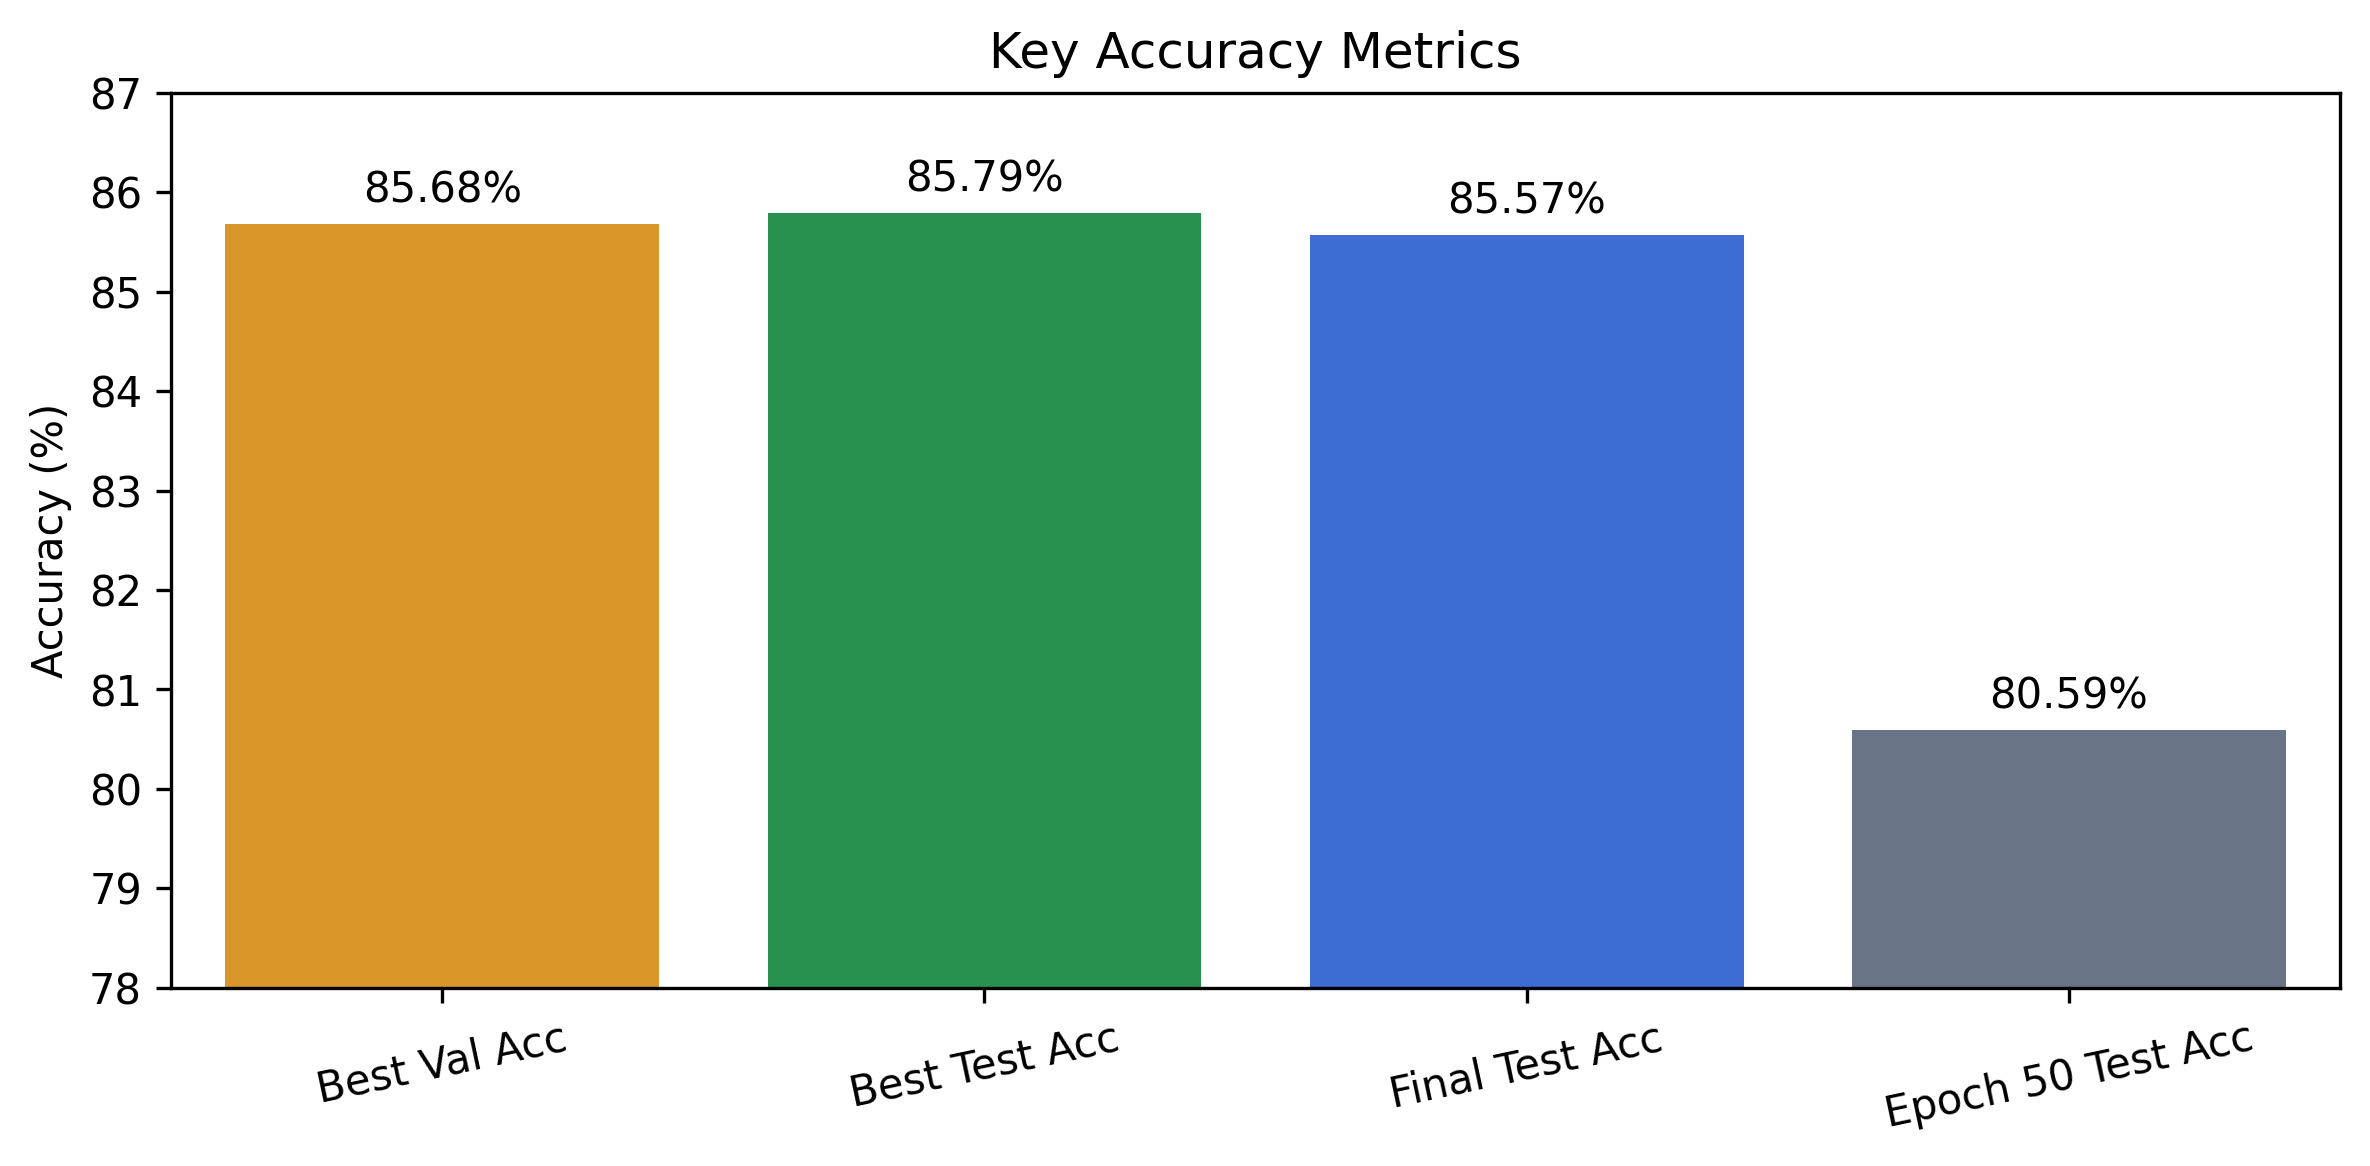
\includegraphics[width=\linewidth]{key_metrics.png}
		\end{column}
		\begin{column}{0.52\textwidth}
			\begin{block}{为什么能超过80\%}
				\begin{itemize}
					\item $4\times4$ patch保留较充分的局部细节
					\item Mixup、RandomErasing、DropPath共同抑制过拟合
					\item EMA与余弦退火提升后期评估稳定性
				\end{itemize}
			\end{block}
			\begin{block}{后期提升变慢}
				模型容量足够，限制主要来自小数据集上的泛化能力；继续训练的收益小于增强和正则化调参。
			\end{block}
		\end{column}
	\end{columns}
\end{frame}

\begin{frame}{总结}
	\begin{block}{完成内容}
		本次实验完成了基于ViT的CIFAR10分类，包括数据增强、Patch Embedding、Transformer Encoder、训练策略、模型保存和日志可视化。
	\end{block}

	\begin{block}{主要收获}
		实践了将图像切分为patch token并送入Transformer的流程，也进一步理解了多头自注意力、位置编码、DropPath、Mixup、EMA和学习率调度的作用。
	\end{block}

	\begin{block}{可改进方向}
		可以继续尝试更强的数据增强、更长训练、更细的patch大小或更系统的正则化参数搜索。
	\end{block}
\end{frame}

\end{document}
